

%% AP Physics MC Questions Archive
%%----------------------------------------


%% Biot Savart
%%----------------------------------------
\element{ap}{
\begin{question}{biot-savart-q01}
    What is the magnetic field due to a wire of infinite length carrying a current $I$,
        a distance $a$ away from the wire?
    \begin{multicols}{3}
    \begin{choices}
      \correctchoice{$\dfrac{\mu_0 I}{2\pi a}$}
        \wrongchoice{$\dfrac{\mu_0 I}{4\pi a}$}
        \wrongchoice{$\mu_0 I$}
        \wrongchoice{$2\pi a \mu_0 I$}
        \wrongchoice{$4\pi a \mu_0 I$}
    \end{choices}
    \end{multicols}
\end{question}
}

\element{ap}{
\begin{question}{biot-savart-q02}
    What is the magnetic field due to a circular loop of wire carrying a current $I$ and having a radius $R$ at the center of the loop?
    \begin{multicols}{3}
    \begin{choices}
        \wrongchoice{$\dfrac{\mu_0 I}{4\pi R}$}
      \correctchoice{$\dfrac{\mu_0 I}{4 R}$}
        \wrongchoice{$\dfrac{\mu_0 I}{2\pi R}$}
        \wrongchoice{$\dfrac{\mu_0 I}{2 R}$}
        \wrongchoice{$2\pi\mu_0 I R$}
    \end{choices}
    \end{multicols}
\end{question}
}

\element{ap}{
\begin{question}{biot-savart-q03}
    The Biot-Savart Law is used to:
    \begin{choices}
        \wrongchoice{determine the electric field created by individual point charges}
        \wrongchoice{determine the electric field created by an electric current}
        \wrongchoice{determine the magnetic field created by individual point charges}
      \correctchoice{determine the magnetic field created by an electric current}
        \wrongchoice{determine the force field created by an electric current}
    \end{choices}
\end{question}
}

\element{ap}{
\begin{question}{biot-savart-q04}
    What is the magnitude of the magnetic force on a semicircle of wire of radius $r$ carrying a current $I$ in the plane of the page due to a uniform magnetic field $B$ pointing out of the page?
    \begin{multicols}{3}
    \begin{choices}
        \wrongchoice{$\pi rIB$}
        \wrongchoice{$rIB$}
      \correctchoice{$2rIB$}
        \wrongchoice{$4rIB$}
        \wrongchoice{$6rIB$}
    \end{choices}
    \end{multicols}
\end{question}
}

\element{ap}{
\begin{question}{biot-savart-q05}
    What is the magnitude and direction of the magnetic field at point $P$ due to the segment of wire above carrying current $I$?
    \begin{center}
    \begin{tikzpicture}
        %% Wire
        \draw[thick,-latex] (3,0) -- (0,0);
        \draw[thick,-latex] (0,0) -- (-3,0);
        %% Current
        \node[anchor=north west] at (0,0) {$I$};
        %% Points P
        \draw[fill] (0,-2) circle (2pt) node[anchor=west] {$P$};
        %% distance d
        \draw (-0.5,0) -- (-0.5,-2) node[pos=0.5,anchor=center,fill=white] {$d$};
        \draw (-0.75,-2) -- (-0.25,-2);
    \end{tikzpicture}
    \end{center}
    \begin{choices}
        \wrongchoice{$\dfrac{\mu_0 I}{2\pi d}$ out of the page}
      \correctchoice{$\dfrac{\mu_0 I}{2\pi d}$ into the page}
        \wrongchoice{$\dfrac{\mu_0 I}{4\pi d}$ out of the page}
        \wrongchoice{$\dfrac{\mu_0 I}{4\pi d}$ into the page}
        \wrongchoice{$\dfrac{\mu_0 I}{d}$ out of the page}
    \end{choices}
\end{question}
}

\element{ap}{
\begin{question}{biot-savart-q06}
    What is the magnitude and direction of the magnetic field at point $P$ due to the segment of wire carrying current $I$?
    \begin{center}
    \begin{tikzpicture}
        %% Wire
        \draw[thick,-latex] (-4,0) -- (-2,0) node[anchor=south east] {$I$};
        \draw[thick] (-2,0) -- (0,0);
        \draw[thick,-latex] (0,0) -- (0,-2);
        \draw[thick] (0,-2) -- (0,-4);
        %% 90 degree
        \draw (-0.25,0) -- (-0.25,-0.25) -- (0,-0.25);
        %% point P
        \draw[dashed] (0,0) -- (2,0) node[pos=0.5,anchor=south] {$d$};
        \draw[fill] (2,0) circle (2pt) node[anchor=south west] {$P$};
    \end{tikzpicture}
    \end{center}
    \begin{choices}
        \wrongchoice{$\dfrac{\mu_0 I}{2\pi d}$ out of the page}
        \wrongchoice{$\dfrac{\mu_0 I}{2\pi d}$ into the page}
      \correctchoice{$\dfrac{\mu_0 I}{4\pi d}$ out of the page}
        \wrongchoice{$\dfrac{\mu_0 I}{4\pi d}$ into the page}
        \wrongchoice{$\dfrac{\mu_0 I}{d}$ out of the page}
    \end{choices}
\end{question}
}

\element{ap}{
\begin{question}{biot-savart-q07}
    What is the magnetic field at point $P$ due to the segment of wire $AB$ carrying current $I$?
    \begin{center}
    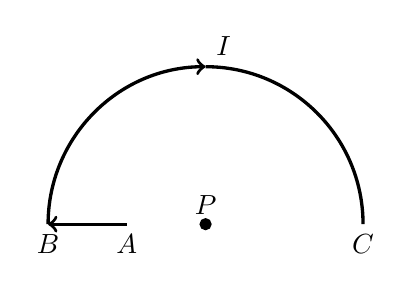
\begin{tikzpicture}
        %% Top Loop
        \draw[very thick,->] (-2,0) arc (180:90:2) node[anchor=south west] {$I$};
        \draw[very thick] (0,2) arc (90:0:2) node[anchor=north] {$C$};
        %% Bottom Straight
        \draw[very thick,->] (-1,0) -- (-2,0)
            node[pos=0,anchor=north] {$A$}
            node[pos=1,anchor=north] {$B$};
        %% Point P
        \draw[fill] (0,0) circle (2pt) node[anchor=south] {$P$};
    \end{tikzpicture}
    \end{center}
    \begin{multicols}{3}
    \begin{choices}
      \correctchoice{zero}
        \wrongchoice{$2\mu_0 Ir$}
        \wrongchoice{$\dfrac{\mu_0}{r}$}
        \wrongchoice{$\dfrac{\mu_0 I}{2r}$}
        \wrongchoice{$\dfrac{\mu_0 I}{4r}$}
    \end{choices}
    \end{multicols}
\end{question}
}

\element{ap}{
\begin{question}{biot-savart-q08}
    Which segments of the wire affect the magnetic field at point $P$ for the above wire?
    \begin{center}
    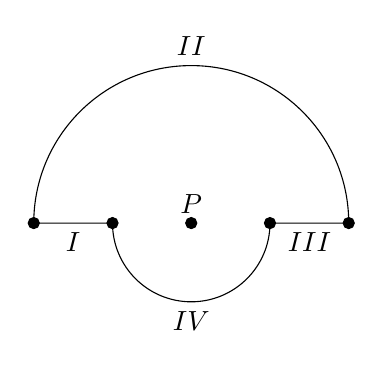
\begin{tikzpicture}
        %% Wire
        \draw (-1,0) -- (-2,0) arc (180:0:2) -- (1,0) arc(360:180:1) -- cycle;
        %% Points
        \draw[fill] (-2,0) circle (2pt);
        \draw[fill] (-1,0) circle (2pt);
        \draw[fill] (0,0) circle (2pt) node[anchor=south] {$P$};
        \draw[fill] (2,0) circle (2pt);
        \draw[fill] (1,0) circle (2pt);
        %% Labels
        \node[anchor=south] at (0,2) {$II$};
        \node[anchor=north] at (-1.5,0) {$I$};
        \node[anchor=north] at (+1.5,0) {$III$};
        \node[anchor=north] at (0,-1) {$IV$};
    \end{tikzpicture}
    \end{center}
    \begin{multicols}{2}
    \begin{choices}
        \wrongchoice{I and III}
      \correctchoice{II and IV}
        \wrongchoice{I, II and III}
        \wrongchoice{II, III and IV}
        \wrongchoice{I, II, III and IV}
    \end{choices}
    \end{multicols}
\end{question}
}

\element{ap}{
\begin{question}{biot-savart-q09}
    Which of the following laws can be used to calculate the magnetic field from an electric current distribution?
    \begin{choices}
        \wrongchoice{Gauss' Law}
        \wrongchoice{Conservation of Charge}
      \correctchoice{Biot-Sarvart Law}
        \wrongchoice{Faraday's Law}
        \wrongchoice{Gauss's Law for Magnetism}
    \end{choices}
\end{question}
}

\endinput


